%%
%% This is file `sample-acmsmall.tex',
%% generated with the docstrip utility.
%%
%% The original source files were:
%%
%% samples.dtx  (with options: `acmsmall')
%% 
%% IMPORTANT NOTICE:
%% 
%% For the copyright see the source file.
%% 
%% Any modified versions of this file must be renamed
%% with new filenames distinct from sample-acmsmall.tex.
%% 
%% For distribution of the original source see the terms
%% for copying and modification in the file samples.dtx.
%% 
%% This generated file may be distributed as long as the
%% original source files, as listed above, are part of the
%% same distribution. (The sources need not necessarily be
%% in the same archive or directory.)
%%
%% Commands for TeXCount
%TC:macro \cite [option:text,text]
%TC:macro \citep [option:text,text]
%TC:macro \citet [option:text,text]
%TC:envir table 0 1
%TC:envir table* 0 1
%TC:envir tabular [ignore] word
%TC:envir displaymath 0 word
%TC:envir math 0 word
%TC:envir comment 0 0
%%
%%
%% The first command in your LaTeX source must be the \documentclass command.
\documentclass[acmsmall,review, nonacm]{acmart}
%% NOTE that a single column version is required for 
%% submission and peer review. This can be done by changing
%% the \doucmentclass[...]{acmart} in this template to 
%% \documentclass[manuscript,screen]{acmart}
%% 
%% To ensure 100% compatibility, please check the white list of
%% approved LaTeX packages to be used with the Master Article Template at
%% https://www.acm.org/publications/taps/whitelist-of-latex-packages 
%% before creating your document. The white list page provides 
%% information on how to submit additional LaTeX packages for 
%% review and adoption.
%% Fonts used in the template cannot be substituted; margin 
%% adjustments are not allowed.
%%
%% \BibTeX command to typeset BibTeX logo in the docs
\AtBeginDocument{%
  \providecommand\BibTeX{{%
    \normalfont B\kern-0.5em{\scshape i\kern-0.25em b}\kern-0.8em\TeX}}}

%% Rights management information.  This information is sent to you
%% when you complete the rights form.  These commands have SAMPLE
%% values in them; it is your responsibility as an author to replace
%% the commands and values with those provided to you when you
%% complete the rights form.
% \setcopyright{acmlicensed}
% \copyrightyear{2024}
% \acmYear{2024}
% \acmDOI{XXXXXXX.XXXXXXX}

%%
%% The majority of ACM publications use numbered citations and
%% references.  The command \citestyle{authoryear} switches to the
%% "author year" style.
%%
%% If you are preparing content for an event
%% sponsored by ACM SIGGRAPH, you must use the "author year" style of
%% citations and references.
%% Uncommenting
%% the next command will enable that style.
%%\citestyle{acmauthoryear}

%% Code listing commands
\usepackage{listings}
\usepackage{xcolor}

% Theme is everforest light from: https://gogh-co.github.io/Gogh/
\definecolor{codegreen}{RGB}{167, 192, 128}
\definecolor{codeblack}{RGB}{75, 86, 91}
\definecolor{codegray}{RGB}{92, 106, 114}
%\definecolor{codepurple}{rgb}{0.58,0,0.82}
\definecolor{backcolour}{RGB}{253, 246, 227}
\definecolor{codeblue}{RGB}{57, 148, 197}


\lstdefinestyle{mystyle}{
    backgroundcolor=\color{backcolour},   
    commentstyle=\color{codegreen},
    keywordstyle=\color{codeblue},
    numberstyle=\tiny\color{codegray},
    %stringstyle=\color{codepurple},
    basicstyle=\ttfamily\scriptsize,
    breakatwhitespace=false,         
    breaklines=true,                 
    captionpos=b,                    
    keepspaces=true,                 
    numbers=left,                    
    numbersep=5pt,                  
    showspaces=false,                
    showstringspaces=false,
    showtabs=false,                  
    tabsize=2,
    xleftmargin=0.3cm,
    frame=tlbr,  
    framerule=0pt,
}

\lstset{style=mystyle}
%%
%% end of the preamble, start of the body of the document source.
\begin{document}

%%
%% The "title" command has an optional parameter,
%% allowing the author to define a "short title" to be used in page headers.
\title{Binary Analysis for Missed Vectorization Opportunities Detection}

%%
%% The "author" command and its associated commands are used to define
%% the authors and their affiliations.
%% Of note is the shared affiliation of the first two authors, and the
%% "authornote" and "authornotemark" commands
%% used to denote shared contribution to the research.
\author{Amos Herz}
\email{amherz@ethz.ch}
\author{Alessandro Legnani}
\email{alegnani@ethz.ch}

\affiliation{%
  \institution{ETH Zürich}
  \city{Zürich}
  \country{Switzerland}
  \postcode{8092}
}

%%
%% By default, the full list of authors will be used in the page
%% headers. Often, this list is too long, and will overlap
%% other information printed in the page headers. This command allows
%% the author to define a more concise list
%% of authors' names for this purpose.
\renewcommand{\shortauthors}{Herz and Legnani}

%%
%% The abstract is a short summary of the work to be presented in the
%% article.
\begin{abstract}
  
\end{abstract}

%%
%% The code below is generated by the tool at http://dl.acm.org/ccs.cfm.
%% Please copy and paste the code instead of the example below.
%%
% TODO: ?
% \begin{CCSXML}
% <ccs2012>
%  <concept>
%   <concept_id>00000000.0000000.0000000</concept_id>
%   <concept_desc>Do Not Use This Code, Generate the Correct Terms for Your Paper</concept_desc>
%   <concept_significance>500</concept_significance>
%  </concept>
%  <concept>
%   <concept_id>00000000.00000000.00000000</concept_id>
%   <concept_desc>Do Not Use This Code, Generate the Correct Terms for Your Paper</concept_desc>
%   <concept_significance>300</concept_significance>
%  </concept>
%  <concept>
%   <concept_id>00000000.00000000.00000000</concept_id>
%   <concept_desc>Do Not Use This Code, Generate the Correct Terms for Your Paper</concept_desc>
%   <concept_significance>100</concept_significance>
%  </concept>
%  <concept>
%   <concept_id>00000000.00000000.00000000</concept_id>
%   <concept_desc>Do Not Use This Code, Generate the Correct Terms for Your Paper</concept_desc>
%   <concept_significance>100</concept_significance>
%  </concept>
% </ccs2012>
% \end{CCSXML}

% \ccsdesc[500]{Do Not Use This Code~Generate the Correct Terms for Your Paper}
% \ccsdesc[300]{Do Not Use This Code~Generate the Correct Terms for Your Paper}
% \ccsdesc{Do Not Use This Code~Generate the Correct Terms for Your Paper}
% \ccsdesc[100]{Do Not Use This Code~Generate the Correct Terms for Your Paper}

%%
%% Keywords. The author(s) should pick words that accurately describe
%% the work being presented. Separate the keywords with commas.
% \keywords{Do, Not, Us, This, Code, Put, the, Correct, Terms, for,
%   Your, Paper}

% \received{20 February 2007}
% \received[revised]{12 March 2009}
% \received[accepted]{5 June 2009}

%%
%% This command processes the author and affiliation and title
%% information and builds the first part of the formatted document.
\maketitle

\section{Introduction}
Modern compilers are often able to automatically vectorize code using 
SIMD instructions.
Take, as an example, the following code snippet: 

\lstinputlisting[caption={\texttt{copy.c}}, label={lst:copy}, language=C]{listings/copy.c}

\noindent We can compile it with the following set of compiler flags
\begin{itemize}
  \item \texttt{-O3}: tells the compiler to use the highest level
        of optimization available.
  \item \texttt{-fno-tree-loop-distribute-patterns}:
        prevents replacing the loop with a call to \texttt{memcpy}
  \item \texttt{-fno-tree-vectorize}: prevents vectorization
\end{itemize}

\noindent Which will produce the following assembly code:

\lstinputlisting[caption={\texttt{copy.c} compiled with vectorizations disabled}, label={lst:copy_compiled}]{listings/copy.s}

\noindent However, by compiling without the \texttt{-fno-tree-vectorize} flag,
the compiler will produce the following vectorized code (note the use of wider instructions and registers):

\lstinputlisting[caption={\texttt{copy.c} compiled with vectorizations enabled}, label={lst:copy_vectorized}]{listings/copy_vectorized.s}

\noindent The main goal of this project is to develop a method for identifying missed opportunities 
for vectorization in existing code. That is, given an existing binary, we want to identify pieces of code
and procedures that could have been vectorized by the compiler but were not.

\section{Related Work}
Autovectorization is \textit{difficult}, compilers tend to miss many optimizations (as shown by \citet{Feng2021})
, and more than often
vectorizing a small piece of code requires large changes to the whole code base 
(as was done for example by \citet{Chen22}).

Compilers have been shown to widely miss out on vectorization opportunities. As an example, \citet{Maleki2021} report that
in their research only 45-71\% of the loops in a benchmark they developed and only a few loops from the real applications 
are vectorized by the compilers they evaluated, which include widely popular compilers such as \texttt{gcc} (version 4.7.0).

Auto-vectorization is still an open field of research: attempts have been made at ``fixing'' the compiler work
by post-processing compiled code (\citet{Porpodas2021}) or by applying Machine Learning to produce improved vectorization schemes
(\citet{Mendis2019}).

\section{Approach}
\subsection{Dataflow Analysis}
Let's look at Listing~\ref{lst:copy_compiled}: there, we can realize that 
the \texttt{load} and \texttt{store} instructions are completely independent (from other instructions of the same type) 
and could, theoretically, be computed in parallel, therefore vectorized. This can be concluded by simply looking at the dataflow,
an example on how a dataflow graph could look like is given in Figure~\ref{fig:dataflow}.

\begin{figure}[h!]
  \includegraphics*[width=0.4\linewidth]{img/dataflow.png}
  \caption{Example of dataflow graph for \texttt{copy.c}}
  \label{fig:dataflow}
\end{figure}

\subsection{Dynamic Analysis}
In order to build a dataflow graph we will be using the dynamic analysis framework 
Intel Pin\footnote{\url{https://software.intel.com/sites/landingpage/pintool/docs/98830/Pin/doc/html/index.html}}.
Intel Pin allows us to instrument single instructions in the assembly to generate 
the appropriate trace information to construct our dataflow graph. 

We opted to use dynamic analysis in our approach as it simplifies the approach of finding missed vectorization when 
compared to static analysis. Dynamic analysis allows us to generate the trace of a given program, containing all of its memory
accesses, which can easily be converted into a dataflow graph.
However, when performing dynamic analysis, we will need to be careful not to falsely report code with 
complex control flow as non-optimized.
\lstinputlisting[caption={\texttt{dyn} function}, label={lst:dyn}, language=C]{listings/dyn.c}
As an example, assume that in an execution of function \texttt{dyn} from Listing \ref{lst:dyn} 
we have that every element of array \texttt{c} is 0. In this case, we would 
observe that \texttt{a = 4 * b} and vectorization would therefore bt trivial.
Therefore, if the code were not to be vectorized, we would flag this code as missing a vectorization opportunity, 
without considering the control flow operation.
Note that this example is actually trivially vectorizable if we were to employ masked 
vector operations. However, this is only an illustrative example and one can consider even more complex control 
flow operations that make the code impossible to be vectorized. 
To fix this issue we can either use static analysis or consider the control flow operation in our dataflow graph.
We plan on using the second approach as it is less complex to implement and are aware of the loss in precision this could result in.

%%Given the trace of execution of a program (instructions and memory accesses), one can build a dataflow graph, on which a dataflow analysis 
%%can be performed to identify  ``parallel'' computations and thus, vectorization opportunities.

All in all, we foresee that building a (correct) dataflow graph will likely be the greatest challenge this project poses. An alternative,
would this challenge turn out to be too big of a one, could be to simply analyze the program trace directly, to track down for example repeating accesses
to increasing (or decreasing) memory addresses that would be vectorizable but are not.

\subsection{Real world examples of missed vectorization opportunities} \label{examples}
By searching on the different bugs and issues trackers of the \texttt{clang} and \texttt{gcc} 
compilers we found two examples where the latest version of a compiler does not 
generate vectorized code. For this we are considering the latests versions of 
both \texttt{gcc} (13.2) and \texttt{clang} (18.1.0).

\subsubsection{Example 1 (\texttt{gcc})}
The following example has been taken from the \texttt{gcc} bugs tracker\footnote{\url{https://gcc.gnu.org/bugzilla/show_bug.cgi?id=96888}}.
\lstinputlisting[caption={Piece of code that \texttt{gcc} fails to vectorize}, label={lst:ex1}, language=C]{listings/ex1.cpp}
One would expect the compiler to generate a mask from the \texttt{word} variable 
and perform masked multiplication to vectorize the code.
Compiling this code with the \texttt{-O3} flag on \texttt{gcc} yields no vectorized code, whereas \texttt{clang} unrolls the inner loop and, 
as expected, makes extensive use of vector instructions. A side-by-side comparison of the two compilers' work can be found 
at the following link: \url{https://godbolt.org/z/W8v4Pc463}.
% \lstinputlisting[caption={\texttt{example1.c} compiled with \texttt{gcc -O3}}, label={lst:ex1_gcc}]{listings/ex1_gcc.S}

\subsubsection{Example 2 (\texttt{clang})}
The following example has been taken from the \texttt{clang} issues tracker\footnote{\url{https://github.com/llvm/llvm-project/issues/74380}}.
\lstinputlisting[caption={Piece of code that \texttt{clang} fails to vectorize}, label={lst:ex2}, language=C]{listings/ex2.cpp}
It appears that when the function in Listing~\ref{lst:ex2} is inlined, \texttt{clang} fails at correctly vectorizing it. However
\texttt{gcc} correctly vectorizes the code without any issue.
A side-by-side comparison of the two compilers' work can be found 
at the following link: \url{https://gcc.godbolt.org/z/x6nEh8oqe}.

\subsection{Test Inputs}
To test our results, we will use code snippets from an already existing autovectorization test suite: \texttt{TSVC}\footnote{https://github.com/UoB-HPC/TSVC\_2}, first described by \citet{Callahan88}.
Other random program generators such as \texttt{YARPGen}\footnote{https://github.com/intel/yarpgen} could be used to generate more, less specific, test inputs, even though
we predict that such less specific inputs could hardly contain code that can be vectorized but is not.

\section{Implementation and Experimental Settings}
As mentioned previously, we will test our implementation (implemented using the latest version of Intel Pin) using the latests versions of 
both \texttt{gcc} (13.2) and \texttt{clang} (18.1.0). In order to do so, we use pieces of code from the \texttt{TSVC} test suite
that are known to be vectorizable, pass them to \texttt{gcc} and \texttt{clang} preventing them to vectorize the resulting binary and then test 
if our implementation can actually spot the (induced) missing vectorization opportunities. 
A diagram representing the pipeline of this project is provided in Figure~\ref{fig:pipeline}.

\begin{figure}[h!]
  \includegraphics*[width=0.9\linewidth]{img/pipeline.png}
  \caption{Sketch of the pipeline of the whole project}
  \label{fig:pipeline}
\end{figure}

As the possibility space of different kinds of missed vectorization opportunities is enourmous we decided to focus on some specific patterns.
Initially our goal will be to be able to recognize basic missed vectorizations, which don't appear ``in the wild'' anymore, like the one shown in Listing~\ref{lst:copy_compiled}. 
To do so more effectively, we will start from the top of the code snippets collection from \texttt{TSVC}\footnote{\url{https://github.com/UoB-HPC/TSVC_2/blob/master/src/tsvc.c}} that contains
various vectorizable pieces of code of increasing complexity, ranging from trivial sum of vectors to more intricated and convoluted operations.

Afterwards we will be focusing on pattern-matching the access patterns found in the two examples described in Section~\ref{examples}, which is non-trivial work.
For this we will be using a our own PinTool to extract the trace and our program 
\texttt{vecspot} to generate the dataflow graph and find missed vectorizations.

\subsection{Current state of the implementation (as of 28.04.2024)}
All the code related to this project can be viewed at the following link: \url{https://github.com/herzamos/ast24-project/}.

At the moment, we are able to correctly instrument the binary code and, leveraging our own PinTool, generate 
a code trace that tracks all the memory accesses (both reads and writes) and basic operations between registers like adds and mults.
On top of that, we can succesfully generate a graph from this trace on which we should be able to perform the dataflow analysis. 
Compiling the code in Listing~\ref{lst:add3}, generating a trace leveraging our 
PinTool and analyzing the trace using our program \texttt{vecspot} we obtain the 
dataflow graph shown in Figure~\ref{fig:add3_dataflow}.

\lstinputlisting[caption={Initial test program for \texttt{vecspot}: \texttt{add3.c}}, label={lst:add3}, language=C]{listings/add3.c}

\begin{figure}[h!]
  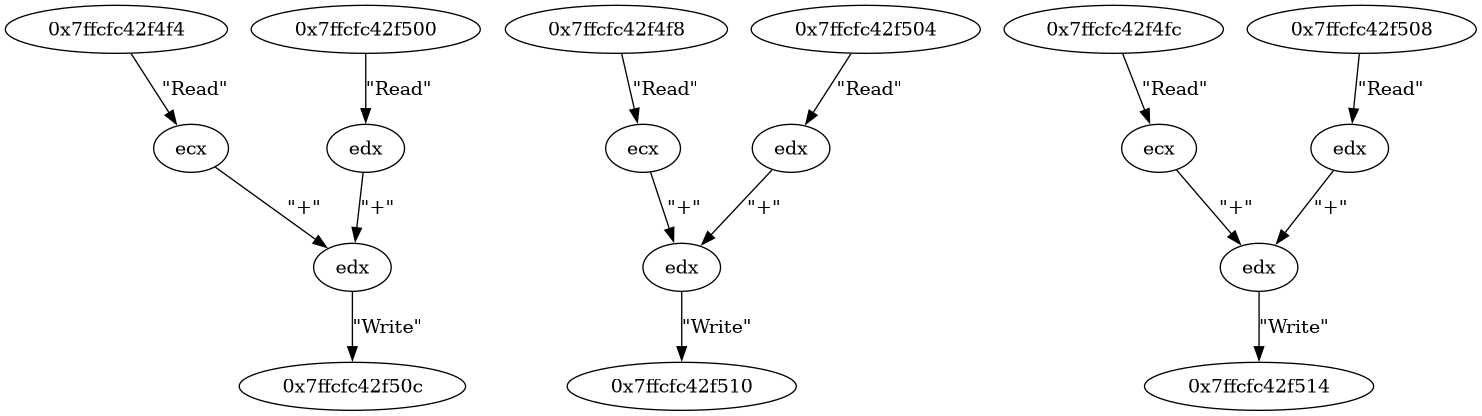
\includegraphics[width=0.9\linewidth]{img/add3.png}
  \caption{Dataflow graph of \texttt{add3.c}}
  \label{fig:add3_dataflow}
\end{figure}

%%
%% The acknowledgments section is defined using the "acks" environment
%% (and NOT an unnumbered section). This ensures the proper
%% identification of the section in the article metadata, and the
%% consistent spelling of the heading.
% \begin{acks}

% \end{acks}

%%
%% The next two lines define the bibliography style to be used, and
%% the bibliography file.
\bibliographystyle{ACM-Reference-Format}
\bibliography{report-references}

%%
%% If your work has an appendix, this is the place to put it.
% \appendix

% \section{Research Methods}

% \subsection{Part One}


% \subsection{Part Two}


% \section{Online Resources}


\end{document}
\endinput
%%
%% End of file `sample-acmsmall.tex'.
